\documentclass{standalone}
\usepackage{tikz}
\usetikzlibrary{shapes,arrows.meta,positioning}

\begin{document}
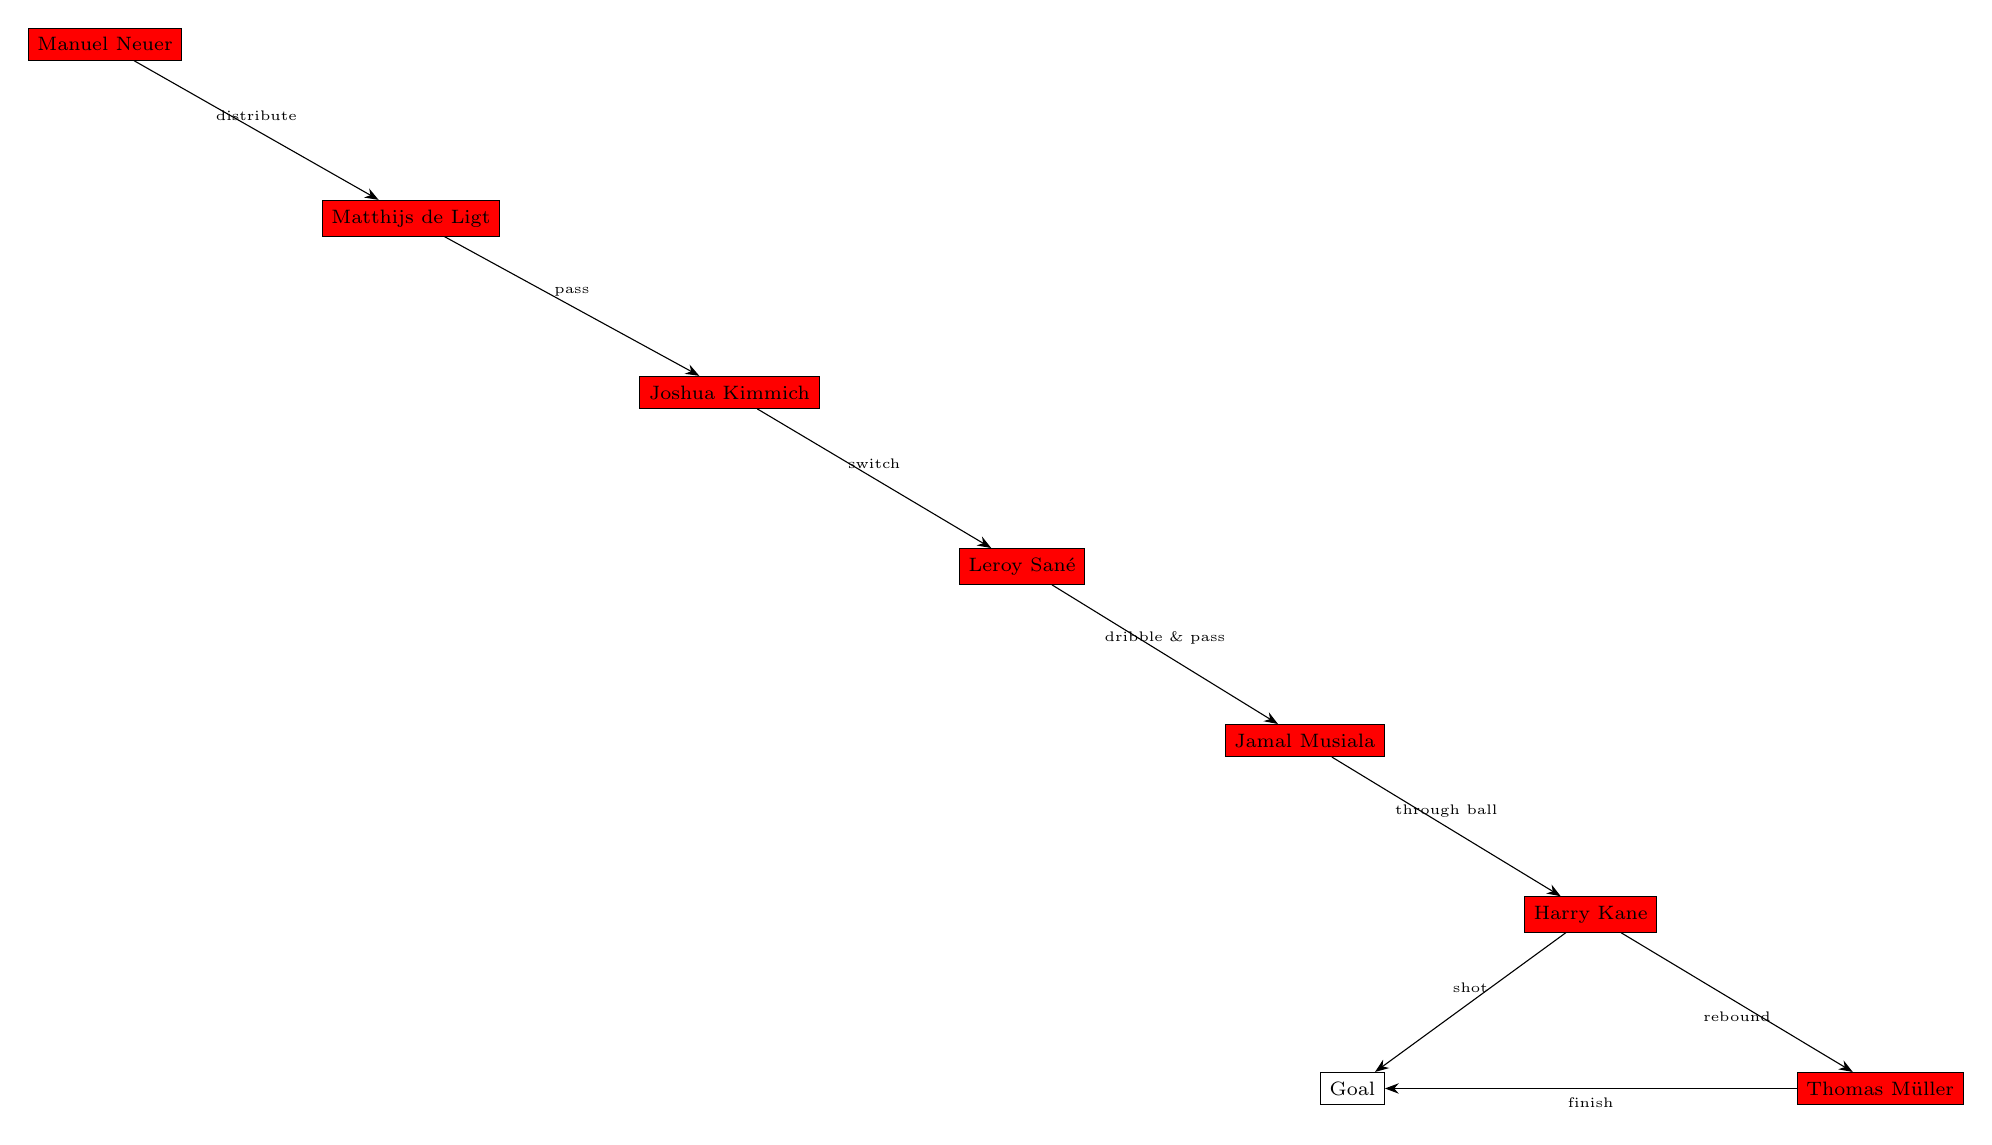
\begin{tikzpicture}[node distance=2.5cm,font=\scriptsize]
    \node[draw,fill=red!100,align=center] (A) {Manuel Neuer};
    \node[draw,fill=red!100,align=center,below right=of A] (B) {Matthijs de Ligt};
    \node[draw,fill=red!100,align=center,below right=of B] (C) {Joshua Kimmich};
    \node[draw,fill=red!100,align=center,below right=of C] (D) {Leroy Sané};
    \node[draw,fill=red!100,align=center,below right=of D] (E) {Jamal Musiala};
    \node[draw,fill=red!100,align=center,below right=of E] (F) {Harry Kane};
    \node[draw,align=center,below left=of F] (G) {Goal};
    \node[draw,fill=red!100,align=center,below right=of F] (H) {Thomas Müller};

    \draw[-{Stealth[length=5pt]},font=\tiny] (A) -- (B) node[midway,above] {distribute};
    \draw[-{Stealth[length=5pt]},font=\tiny] (B) -- (C) node[midway,above] {pass};
    \draw[-{Stealth[length=5pt]},font=\tiny] (C) -- (D) node[midway,above] {switch};
    \draw[-{Stealth[length=5pt]},font=\tiny] (D) -- (E) node[midway,above] {dribble \& pass};
    \draw[-{Stealth[length=5pt]},font=\tiny] (E) -- (F) node[midway,above] {through ball};
    \draw[-{Stealth[length=5pt]},font=\tiny] (F) -- (G) node[midway,above] {shot};
    \draw[-{Stealth[length=5pt]},font=\tiny] (F) -- (H) node[midway,below] {rebound};
    \draw[-{Stealth[length=5pt]},font=\tiny] (H) -- (G) node[midway,below] {finish};
\end{tikzpicture}
\end{document}